\chapter{Literature Review}\label{chapter2}

In this section, a overview of relevant literature and terminology will be reviewed. Common models, methods and studies will be examined and discussed in a critical manner. The background and the problem definition will introduce and help motivate the domains of the research mentioned in the following sections. The purpose is to demonstrate the field(s) related to the \dimsum task and relevant literature for creating a state-of-the-art solution.

The use of Semantic supersenses along with Multiword Expressions (MWE) will be introduced. The supersenses will demonstrate a model for organising broad semantic tagging while MWEs will encapsulate phrasal level entities in discourse models.

Initially, The problem definition will describe the formulation of the task and its motivations on a deeper level. The review section describes the relevant background information which is prevalent in the field of topics to \dimsum. It will contain various descriptions of key terminology followed by an overview of case studies on the corresponding model domain. The related tasks section will cover relevant research in the domain associated with the project. Finally, the discussion gives motivation for the model that will be used to accomplish the task.

\section{Background}

Word level definitions have historically been described in prose using dictionaries. The thesaurus was its historical counterpart for synonyms are related terms such as antonyms. In the semantic domain, synonymy is not considered perfect, meaning two words are never considered perfectly equivalent in meaning. The study of this word level meaning has been called Lexical semantics.

Meaning and form have always considered to have a relationship. Semantics can be studied as a strict lexical field but most systems incorporate syntactic form to create rich and robust model. Using syntactic class information such as POS tags, form can help elucidate meaning. Initial studies such as Named Entity Recognition were concerned only with nominals, using tag sequences to demarcate contextual limits. 

Recognising that compositionality does not apply to idiomatic phrases\footnote{``...the meaning of an idiom cannot be predicted on the basis of a knowledge of the rules that determine the meaning or use of its parts...'' \cite{nunberg1994idioms}} leads to more formal definitions of Multiword Expressions. Structure and lexicon are now used in conjunction to help recognise phrasal level entities as lexical in nature. 

Most if not all NLP tasks must consider ambiguity on word and phrase level to make robust and scalable systems. Lexical semantics must then consider disambiguation of meaning from a word sense level to a multiword domain. Word sense disambiguation paired with Multiword expressions leads to a difficult yet broad set of problems to be explored.

\dimsum is such a task, which tries to recognise Multiword Expression boundaries and assign semantic labels within a body of text.

\subsection{Problem Definition}

The difficulty in defining a system is qualifying what constitutes ``good''. One could say it is an elegant and generalised solution that is robust; flexible and accurate, able to recognise new form and meaning in novel situations. In regards to the task at hand, there are two main parts to consider. Correct demarcation of MWE boundaries and correct assignment of Supersenses to any and all potential targets, being words or MWEs alike.

The \dimsum task tries to create a structure which has broad-coverage of the minimal semantic units in the dataset by using semantic supersenses. Lexical units will be tagged with their corresponding supersense while other expressions will be grouped into MWEs and labelled as single semantic units. Additional things to consider are robust boundary demarcation of contiguous and long range dependencies in MWEs.

Quantifying a robust system in the domain of \dimsum entails maintaining a F1-Score within the original publication's results\footnote{Between 25.71\% to 57.77\% as seen in Section \ref{chapter5resultscomparisons}}.

\section{Review}

In this section, studies related to \dimsum will be reviewed in such a way as to give historical context and motivation. 

\subsection{Foundations}
\subsection{Multiword Expressions}\label{mwe}

Recognition and disambiguation of Multiword Expressions is a key issue in NLP, but a reliable definition is paramount to creating a reliable solution for \dimsum. The principle of compositionality\footnote{Generally attributed to Friedrich Ludwig Gottlob Frege} states that ``the principle that the meaning of a complex expression is determined by the meanings of its constituent expressions''\cite{wiki:Principle_of_compositionality}. This is clearly not the case for Multiword Expressions as their constituent parts infrequently correspond to their composed meaning. To overcome this, compositionality of MWEs were initially treated as ``words with spaces'' which could not capture all forms, therefore more in depth definitions were formed by \cite{Sag2002}. 

MWEs are usually defined in a strong (non-compositional) and weak (compositional) sense. From the strongest to the weakest are: {\bf Fixed Expressions} and {\bf Institutionalised Phrases},  {\bf Semi-Fixed Expressions},  {\bf Syntactically-Flexible Expressions}. The definitions are used to clarify types and usage of MWEs but in the \dimsum task, MWEs are only defined as strong (without ``gaps'') or weak (with ``gaps''). Summarising, ``Gappy'' constructions would then be considered {\bf Semi-Fixed Expressions} and {\bf Syntactically-Flexible Expressions} while those without are {\bf Fixed Expressions} and {\bf Institutionalised Phrases}.

\subsubsection{Supersenses}\label{supersenses}
Classification of unknown or unseen words into semantic labels is paramount for generalising language. WordNet was developed as a ``lexical database for English''\cite{Miller1995} and its usage is far reaching and provides a rich dataset framework for many semantic tasks. The usage of supersenses are usually derived from the most broad word sense which describes a set of corresponding terms. A {\it hypernym} is a parent term whose semantic sense encapsulates the concept of another, while a {\it hyponym} is its child, a more specific term. By reviewing the hyponym / hypernym relationship, we can determine broad senses which are useful for describing related terms. 

\begin{figure}[!htbp]
\centering
 \begin{framed}
  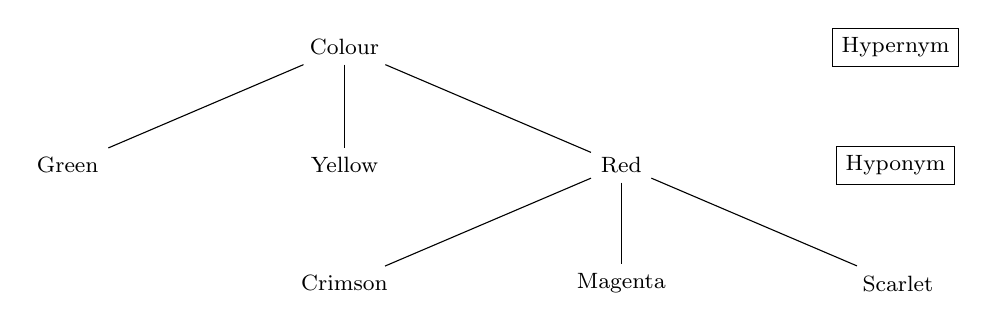
\begin{tikzpicture}[sibling distance=10em,
    every node/.style = {align=center}]]
    \node[draw] at (7,0) {Hypernym};
    \node[draw] at (7,-1.5) {Hyponym};
    \node {Colour}
    child { node {Green} }
    child { node {Yellow} }
    child { node {Red}
      child { node {Crimson} }
      child { node {Magenta} }
      child { node {Scarlet} }
    };
  \end{tikzpicture}
 \end{framed}
\caption{An example hypernym / hyponym hierarchy}
\label{fig:hyptree}
\end{figure}

Using different colours as an example, Figure \ref{fig:hyptree} shows the relationship of a hypernym parent and its hyponym child in a tree representation.

We can traverse a hypernym chain of parent nodes and determine a list of {\bf Semantic {\it Supersenses}}. Using top level word senses is the general methodology for creating a broad coverage supersense set of terms. WordNet has a closed set of top level hypernyms or supersenses which are used for broad coverage semantic word sense classification.

\begin{table}[!htbp]
  \centering
  \begin{tabular}{ |llll| }
    \hline
    n.Tops & n.act & n.animal & n.artefact\\
    n.attribute & n.body & n.cognition & n.communication\\
    n.event & n.feeling & n.food & n.group\\
    n.location & n.motive & n.object & n.person\\
    n.phenomenon & n.plant & n.possession & n.process\\
    n.quantity & n.relation & n.shape & n.state\\
    n.substance & n.time & v.body & v.change\\
    v.cognition & v.communication & v.competition & v.consumption\\
    v.contact & v.creation & v.emotion & v.motion\\
    v.perception & v.possession & v.social & v.stative\\
    v.weather & \  & \  & \ \\
    \hline
  \end{tabular}
  \caption{Noun and Verb Supersenses}
  \label{tab:wordnetsupersenses}
\end{table}

Table \ref{tab:wordnetsupersenses} shows the 41 top level Noun and Verb supersenses from WordNet. A generalised taxonomy of verbs and nouns is useful to broaden semantic scope. Using dictionaries for supervised learning by \cite{ciaramita2003supersense} introduced a framework of closed set supersenses which generalised well for unseen Named entities. 

The foundation for MWE and Supersense corpus was from hand-annotated Wikipedia articles performed by \cite{Schneider2012} which used a limited set of ``topics'' but relied heavily on expert knowledge by inexperienced annotators. These initial conclusions about broad supersense coverage motivates further broad class studies. Sequence tagging with an extended supersense set was interpreted as a type of Word Sense Disambiguation (WSD) task performed by \cite{Ciaramita2006} modifying the HMM model by \cite{collins2002discriminative}. Exploiting the POS tags syntactic context and the historical methodologies for sequence tagging proved to be an important baseline and ``offer a middle ground in granularity'' to generalise named entity classes and verbs\cite{Schneider2016}.

Supersenses in WordNet cover only nouns and verbs whereas adjectives do not have any type of hierarchical relationship. Additional studies extended taxonomic hierarchies to adjectives as performed by \cite{Tsvetkov2014} by using weakly supervised learning methods and crowdsourcing techniques. 

In addition, supersense tagged data corpora created using weakly supervised methodologies have been covered by \cite{Johannsen2014} and \cite{Owoputi2012} with the latter being provided \cite{dimsum16webdata} for use in the \dimsum shared task\cite{dimsum16web}. 

Supersenses by design are lexically assigned, coupled with a definition of MWEs, implies that Supersenses are just like other lexical items: Any single MWE can be assigned a Supersense.

\subsubsection{Word-Sense Disambiguation}

A dictionary entry, or ``citation form'' is referred to as a {\it lemma} in lexical semantics. A {\it lemma} can of course have many meanings referred to as {\it word senses} such as ``water'' meaning {\it liquid form of ${H_2}O$} or {\it to irrigate}. These {\it lemma} of multiple meanings are called {\it homonyms}. Being able to disambiguate a {\it word sense} in its context is referred to as {\bf Word-Sense Disambiguation}.
On the other hand, {\it Polysemy} is when the {\it word senses} are related in meaning. In addition to our previous example, ``water'' can also refer to a {\it body of water} such as ``the water is rough today'' when speaking about the ocean waves. These meanings of ``water'' could be said to be {\it Polysemous} since they both refer to {\it liquid ${H_2}O$} in some form, be it small or large. For readability, differing {\it word senses} are usually written with a superscript integer.

\begin{figure}[!htbp]
\centering
\begin{framed}
\begin{minipage}{.5\textwidth}
\centering
  \begin{tabular}{ | l | l | l |}
    \hline
    Sense & POS & Meaning\\
    \hline
    $Water^1$ & Noun & $H2O$\\
    $Water^2$ & Noun & body of water\\
    $Water^3$ & Verb & to irrigate\\
    \hline
  \end{tabular}
\end{minipage}\hfill
\begin{minipage}{.5\textwidth}
 \centering
 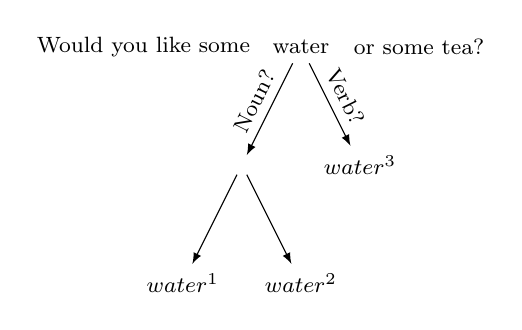
\begin{tikzpicture}
  [
    edge from parent/.style = {draw, -latex},
    every node/.style       = {font=\footnotesize},
    sloped
  ]
 \node at (-2,0) {Would you like some};
 \node at (1.5,0) {or some tea?};
 \node {water}
  child { node  {}
  child { node {$water^1$}}
  child { node {$water^2$}} edge from parent node [above] {Noun?} }
  child { node {$water^3$} edge from parent node [above] {Verb?} };
 \end{tikzpicture}
\end{minipage}
\end{framed}
\caption{An example WSD diagram}
\label{fig:decisionwsd}
\end{figure}

Figure \ref{fig:decisionwsd} shows a word sense table and decision tree representing the disambiguation choice by a computer system for an isolated word. Most modern systems do not make a singular choice in WSD tasks but rather use contextual or sequential information for word sense classification.

In addition to the traditional word disambiguation tasks, additional ``All-words'' WSD tasks have been proposed and studied. Instead of determining a specific word sense, systems learn all word senses and disambiguate in a larger phrasal context, such as sentence level\cite{Stetina1998}. Work by \cite{Ye2007} used Maximum Entropy models for preposition sense disambiguation which contrasted a type of BOW\footnote{Bag-Of-Words} model with surrounding POS tag information. Its results showed that ``collocation-based features'' were the most informative. Similar methodologies and results were done by \cite{Tratz2010} for nominals. 

\subsubsection{WSD and MWE}

Assigning supersenses to MWEs requires the ability to disambiguate their meaning from other potential meanings. This could occur due to syntactic ambiguity, inconsistent compositional parsing or competing context. While lexical ambiguity is more fine grained, both suffer from similar issues in Word Sense Disambiguation tasks. To disambiguate, we must have a sense of semantic relatedness, or semantic distance. Determining the most related sense should yield the obvious unambiguous conclusion for a given word. Semantic relatedness can be interpreted in statistical model, sequential, hierarchical or in graphs. Therefore distance can be determined given a model. There are many competing models but the initial heuristic for WSD systems is generally considered to be first-sense or predominant sense. A naive system which defaults to first-sense is used to determine the baseline capacity of a system. Considerable effort has been put into creating a reliable mechanism for evaluation such as methodologies developed by \cite{Lesk1986}. It hypothesised that observing textual context demonstrates relations which can be disambiguated using dictionaries.

In the Unsupervised All-words WSD using grammatical dependencies by \cite{Nastase2008}, a directed graph is used to determine word senses using the British National Corpus (BNC). Weights are placed on the edges and traversed to a root node, the best scoring path is used to disambiguate the word sense. The graph was created using a mixture of grammatical information for filtering interconnected nodes and semantic relations using the Word Sketch Engine\cite{Kilgarriff2014}. It also compared tie-breaking techniques for sense selection using PageRank and Lesk-based similarity. It showed that using grammatical constraints limit word-sense comparisons and help ``estimate selectional preference from an untagged corpus''\cite{Nastase2008}.

Most WSD tasks focus on the ability to disambiguate nouns and verbs. In the study by \cite{Hovy2010}, experiments of parameter choices for preposition disambiguation were analysed within its syntactic domain. Contextual dependencies of nouns, verbs and adjectives were observed in a fixed and selective window sizes to alleviate issues with conflation and sparsity. Prepositional phrases were labelled with one of seven classes and disambiguated using a Maximum Entropy model. Broader fixed window sizes showed higher accuracy, implying larger context has more semantic information. This idea is prevalent within the field and in line with the ``opaque mask'' formulation by \cite{weaver1955} stating ``if N is large enough one can unambiguously decide the meaning of the central word''. Interestingly, a selective dynamic window size based on syntactic heuristics performed better, outperforming \cite{OHara2009} which used only Fixed-window size.

A multilingual evaluation of techniques to automatically acquire MWEs from corpora was explored by \cite{Ramisch2012} which showed that the techniques with higher coverage of nominals had lower precision while higher precision techniques were inflexible. Alternative machine learning methodologies were suggested which could potentially play to the strengths for both approaches. 

A multilingual study used English resources to extend to foreign languages by detecting whether an MWE is a metaphor. \cite{Tsvetkov2013} used a methodology described as Common Semantic Features (CSF). It used a set of features in English to classify sentences as literal or metaphoric. The three features used included WordNet lexicographer file names, Vector Space Models to compute abstractness/concreteness and Named Entity types. Entities were recognised as SVO\footnote{Subject-Verb-Object} objects which used logistic regression to create a binary classifier. The algorithm was trained with English and evaluated on Russian. Interestingly, the difference in $F_1$ scores was within 2 percent for the Russian Model. Their claim was that semantic features are common as opposed to lexical features which are not, therefore the model could generalise well on Russian. The mixed feature based system created a rich and robust set of quantifiable concepts into a single algorithm but I have doubts that the model would generalise well on languages that have drastically different syntactic structures\footnote{Such as VSO languages like Gaelic or Tagalog}.

Many studies focus on a specific subset of MWE constructions, a broad coverage of entity constructions were covered by \cite{Schneider2014}. It used a rich and robust annotated social web corpus \cite{Schneider2014a} which is derived from the English Web Treebank \cite{bies2012english}. By using the structured perceptron with cost augmentation and features that recognise ``gappy'' structures, the task was one of the first supervised learning systems to identify heterogeneous MWEs. It has the ability to recognise strong and weak MWE constructions. Additional enhancements were introduced and implemented in the subsequent study \cite{Schneider2015} which added supersenses. This final study represents a state-of-the-art system for MWE recognition using supersenses \cite{Schneider2015}.
  
\subsubsection{Sequence labelling and Structured Prediction}

The \dimsum task can be interpreted as a sequence labelling task or a general structured prediction task. In the case of this dissertation, it is treated as such.

Sequence label prediction tasks such as POS tagging concentrate on sequential syntactic recognition in natural language processing. POS tagging systems are considered to have broad coverage for introduction of novel words within a contextual environment.

\begin{table}[!htbp]
  \centering
  \begin{tabular}{ lllllllll }
    The & man & in & the & black & shirt & trades & pokemon & cards\\
    \hline
    DT & NN & IN & DT & JJ & NN & VBZ & JJ & NNS\\
  \end{tabular}
  \caption{A POS Tagged Sentence}
  \label{tab:postagseq}
\end{table}

Table \ref{tab:postagseq} shows a POS tagged sequence\footnote{taken from the Stanford Natural Language Inference (SNLI) dataset \cite{bowman2015large}} which uses the Penn Treebank tagset\cite{Marcus1993}. The use of Hidden-Markov Models (HMM) for POS tagging\cite{Collins2002} has lead to reliable sequence tagging systems. If modelled properly, robust systems can tag unseen words, maintaining a minimum 85\% accuracy for the last decade \cite{brants2000tnt}. Creating methodologies for accurate POS tagged sentences laid the foundation for structured prediction labelling tasks.

\begin{figure}[H]
  \tikzset{font=\footnotesize}
  \centering
  \begin{tikzpicture}[->,>=stealth',shorten >=1pt,auto,node distance=2.8cm,semithick,text width=1.4cm, align=center]
    \node[state] (A)              {the};
    \node[state] (B) [right of=A] {area};
    \node[state] (C) [right of=B] {and};
    \node[state] (D) [right of=C] {Fuji};
    \node[state] (E) [right of=D] {Sushi};
    \node[state] (F) [below of=A] {DET};
    \node[state] (G) [below of=B] {NOUN};
    \node[state] (H) [below of=C] {CONJ};
    \node[state] (I) [below of=D] {PROPN};
    \node[state] (J) [below of=E] {PROPN};

    \path
    (A) edge              node {} (B)
    (A) edge              node {} (F)
    (B) edge              node {} (C)
    (B) edge              node {} (G)
    (C) edge              node {} (D)
    (C) edge              node {} (H)
    (D) edge              node {} (E)
    (D) edge              node {} (I)
    (E) edge              node {} (J);
  \end{tikzpicture}
  \caption{Example HMM with POS tags from \dimsum data}
  \label{fig:hmmposdimsum}
\end{figure}

Named Entity Recognition (NER) was historically viewed as a type of Information Retrieval (IR) task but theoretically could be considered a specific subset of Multiword Expressions. Exploiting the tagging of nominals and augmenting structures with BIO-style\cite{Ramshaw1994} information leads to the ability to recognise {\bf B}eginning, {\bf I}nside and {\bf O}utside points in a Named Entities which is extended to be used in \dimsum for Multiword Expressions.

\begin{table}[!htbp]
\small
\begin{framed}
 \begin{tabular}{lllllllll}
  American & Airlines & , & a & unit & of & AMR & Corp. & ,\\ 
  NNP & NNPS & PUNC & DT & NN & IN & NNP & NNP & PUNC \\
  $B_{NP}$ & $I_{NP}$ & $O$ & $B_{NP}$ & $I_{NP}$ & $B_{PP}$ & $B_{NP}$ & $I_{NP}$ & $O$
 \end{tabular}\\ \ \\

 \begin{tabular}{llllllllll}
  immediately & matched & the & move & , & spokesman & Tim & Wagner & said & .\\
  RB & VBD & DT & NN & PUNC & NN & NNP & NNP & VBD & PUNC\\
  $B_{ADVP}$ & $B_{VP}$ & $B_{NP}$ & $I_{NP}$ & $O$ & $B_{NP}$ & $I_{NP}$ & $I_{NP}$ & $B_{VP}$ & $O$
 \end{tabular}
\end{framed}
 \caption{Sentence with BIO encoding and POS tags}
 \label{tab:biotagseq}
\end{table}

Table \ref{tab:biotagseq} shows an example POS tagged sentence with BIO encoding taken from an example in \cite{martin2000speech}. NER tasks can be therefore thought of as a subsumed precursor to Multiword Expression recognition tasks as NER sequences are contiguous while MWEs are syntactically flexible.

Work on ``exploiting syntactic forms'' by ``token classification of potential idioms'' \cite{Cook2007} intended to use features recognised in a narrow syntactic domain using Unsupervised learning to determine components as idiosyncratic. It proved to perform within a very narrow margin of error in comparison to its supervised counterparts (within 4\%) which were more concerned with a compositional approach. This type of syntactic narrow scope proved to be important in building informative generalisations. More modern studies show the relationship can be modelled simultaneously. Using Conditional Random Fields (CRF) by \cite{Constant2011} showed the ability to broaden the domain of NER to recognise noun and verb like idiomatic phrases.

Although syntactic information gives structure to sequences, a higher semantic scope is needed to broaden the context and generalise well. A overarching set of word senses are needed to encapsulate lexical and phrasal MWEs\footnote{Definitions of MWE types can be seen in section \ref{mwe}}. WordNet \cite{fellbaum1998wordnet} introduced a lexical database allowing generalisation into broad semantic supersenses.

Interpreting \dimsum as a structured prediction task we can broaden our model scope. Initial work using Conditional Random Fields (CRF) by \cite{lafferty2001conditional} and \cite{Collins2002} showed that sequence prediction using CRFs is possible and quite powerful, producing state-of-the-art results at the time.

As opposed to HMMs as seen in Figure \ref{fig:hmmposdimsum}, CRFs have the benefit of being able to use any input for label prediction. In Figure \ref{fig:crfwindowdimsum} we can see the current input \texttt{O} using a window size of 2 on either side for feature extraction.

\begin{figure}[H]
  \centering
  \tikzset{font=\footnotesize}
  \begin{tikzpicture}[-,>=stealth',shorten >=1pt,auto,node distance=2.8cm,semithick,text width=1.3cm, align=center]
    \node[state] (A)              {$y_0$};
    \node[state] (B) [right of=A] {$y_1$};
    \node[state] (C) [right of=B] {$y_2$};
    \node[state] (D) [right of=C] {$y_3$};
    \node[state] (E) [right of=D] {$y_4$};
    \node[state] (F) [below of=A] {$x_1$};
    \node[state] (G) [below of=B] {$x_2$};
    \node[state] (H) [below of=C] {$x_3$};
    \node[state] (I) [below of=D] {$x_4$};
    \node[state] (J) [below of=E] {$x_5$};

    \path
    (A) edge              node {} (B)
    (A) edge              node {} (F)
    (B) edge              node {} (C)
    (B) edge              node {} (G)
    (C) edge              node {} (D)
    (C) edge              node {} (H)
    (D) edge              node {} (E)
    (D) edge              node {} (I)
    (E) edge              node {} (J);

    \path[draw, densely dotted]
    (C) edge              node [midway,above,sloped]{-2} (F)
    (C) edge              node [midway,above,sloped]{-1} (G)
    (C) edge              node [midway,above,sloped]{+1} (I)
    (C) edge              node [midway,above,sloped]{+2} (J);
  \end{tikzpicture}
  \caption{Example CRF showing $\pm$2 Window}
  \label{fig:crfwindowdimsum}
\end{figure}

Similar to the \dimsum task using Linear Chain CRFs a type of POS and MWE tagger by \cite{Constant2011} used different and smaller set of predefined senses. Moving towards the state of the art introduced the WordNet Supersenses while recognising syntactically flexible constrictions by \cite{Schneider2014}. The original \dimsum task publication mentions that two of the top three systems use CRFs for structured prediction. In fact, the baseline solution spoken of in Chapter \ref{chapter4} uses a CRF due to its proven track record in positive results. 

Many modern structured prediction systems are moving away from featured engineered systems with a preference towards a purely data driven model. Initial studies by \cite{collins2002discriminative} of a Structured perceptron prove the ability of multi-class labelling in the framework of POS tagging. By using a Neural Network approach, weights are optimised by learning from training data. Deep Neural Networks (DNN) have the ability to discriminate non-linearly allowing for non-binary labelling. \dimsum requires such capabilities are all label predictions are multi-class. Figure \ref{fig:nndiagram} shows a Neural Network with a Neuron and Activation layer\footnote{Original TikZ picture created by \cite{neuralnetdiagram}}.

%Neural Network
\begin{figure}[H]
\begin{tikzpicture}[
plain/.style={
  draw=none,
  fill=none,
  },
net/.style={
  matrix of nodes,
  nodes={
    draw,
    circle,
    inner sep=10pt
    },
  nodes in empty cells,
  column sep=2cm,
  row sep=-9pt
  },
>=latex
]
\matrix[net] (mat)
{
|[plain]| \parbox{1.3cm}{\centering Input\\layer} & |[plain]| \parbox{1.3cm}{\centering Hidden\\layer} & |[plain]| \parbox{1.3cm}{\centering Output\\layer} \\
& |[plain]| \\
|[plain]| & \\
& |[plain]| \\
|[plain]| & |[plain]| \\
& & \\
|[plain]| & |[plain]| \\
& |[plain]| \\
|[plain]| & \\
& |[plain]| \\
};
\foreach \ai [count=\mi ]in {2,4,...,10}
  \draw[<-] (mat-\ai-1) -- node[above] {Input \mi} +(-2cm,0);
\foreach \ai in {2,4,...,10}
{\foreach \aii in {3,6,9}
  \draw[->] (mat-\ai-1) -- (mat-\aii-2);
}
\foreach \ai in {3,6,9}
  \draw[->] (mat-\ai-2) -- (mat-6-3);
\draw[->] (mat-6-3) -- node[above] {Output} +(2cm,0);
\end{tikzpicture}

\begin{tikzpicture}[
init/.style={
  draw,
  circle,
  inner sep=2pt,
  font=\Huge,
  join = by -latex
},
squa/.style={
  draw,
  inner sep=2pt,
  font=\Large,
  join = by -latex
},
start chain=2,node distance=13mm
]
\node[on chain=2] 
  (x2) {$x_2$};
\node[on chain=2,join=by o-latex] 
  {$w_2$};
\node[on chain=2,init] (sigma) 
  {$\displaystyle\Sigma$};
\node[on chain=2,squa,label=above:{\parbox{2cm}{\centering Activate \\ function}}]   
  {$f$};
\node[on chain=2,label=above:Output,join=by -latex] 
  {$y$};
\begin{scope}[start chain=1]
\node[on chain=1] at (0,1.5cm) 
  (x1) {$x_1$};
\node[on chain=1,join=by o-latex] 
  (w1) {$w_1$};
\end{scope}
\begin{scope}[start chain=3]
\node[on chain=3] at (0,-1.5cm) 
  (x3) {$x_3$};
\node[on chain=3,label=below:Weights,join=by o-latex] 
  (w3) {$w_3$};
\end{scope}
\node[label=above:\parbox{2cm}{\centering Bias \\ $b$}] at (sigma|-w1) (b) {};

\draw[-latex] (w1) -- (sigma);
\draw[-latex] (w3) -- (sigma);
\draw[o-latex] (b) -- (sigma);

\draw[decorate,decoration={brace,mirror}] (x1.north west) -- node[left=10pt] {Inputs} (x3.south west);
\end{tikzpicture}
\caption{Diagram of a Neural Network and a Neuron}
\label{fig:nndiagram}
\end{figure}

One of the main issues with NNs is that long term dependencies are not captured well as weights are optimised over an entire training set. Long term dependencies are not ``remembered'' where as Recurrent Neural Networks (RNN) fix this issue. Long-Short Term Memory (LSTM) RNNs have additional weights and feedback mechanisms for capturing long term dependencies and ``remembering'' potentially useful information for discriminate labelling tasks. These feedback mechanisms can be thought of as a loop in a Neural Network or alternatively an unrolled sequence of RNNs as seen in Figure \ref{fig:rnnunrolled}\footnote{Figure taken from \cite{understandinglstmolah}}.

%Unrolled LSTM Image
\begin{figure}[H]
\centering
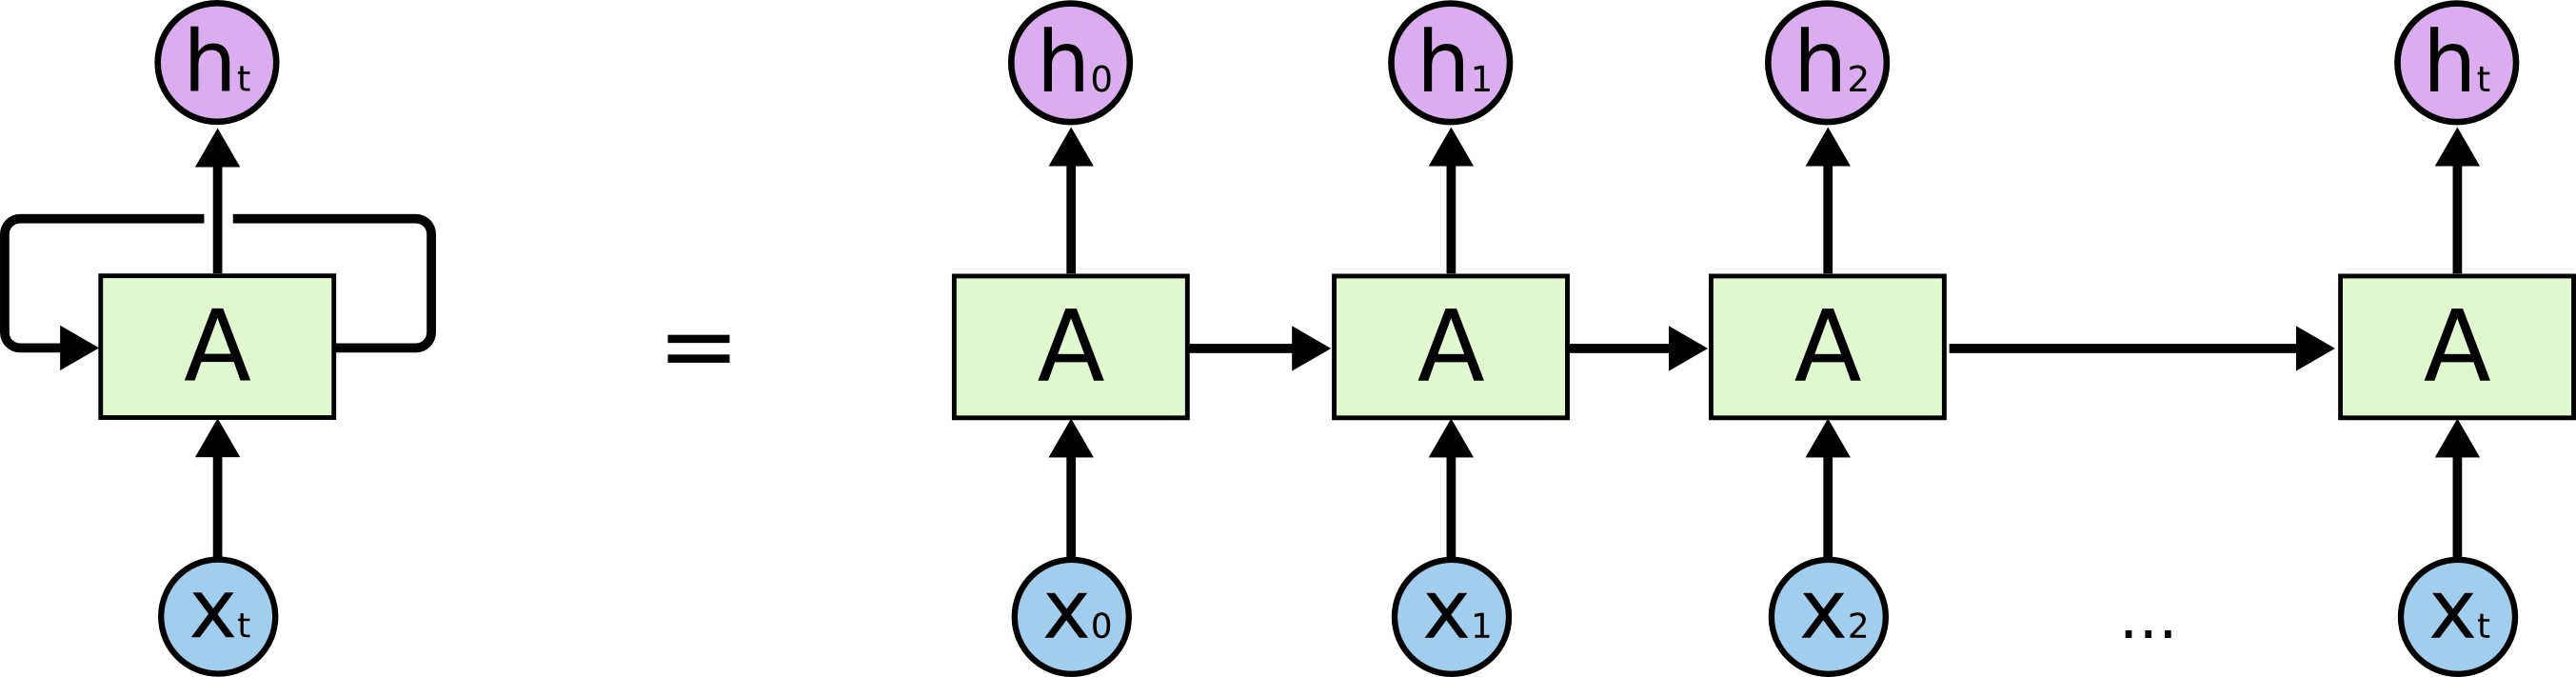
\includegraphics[width=0.8\textwidth]{images/RNN-unrolled.png}
\caption{Unrolled RNN}
\label{fig:rnnunrolled}
\end{figure}

Unlike a neural network's neuron, there are multiple non-linear activation functions which work together to ``remember'' details that would otherwise be forgotten in other DNNs as seen in Figure \ref{fig:lstmcell}\footnote{Figure taken from \cite{understandinglstmolah}}.

\begin{figure}[H]
\centering
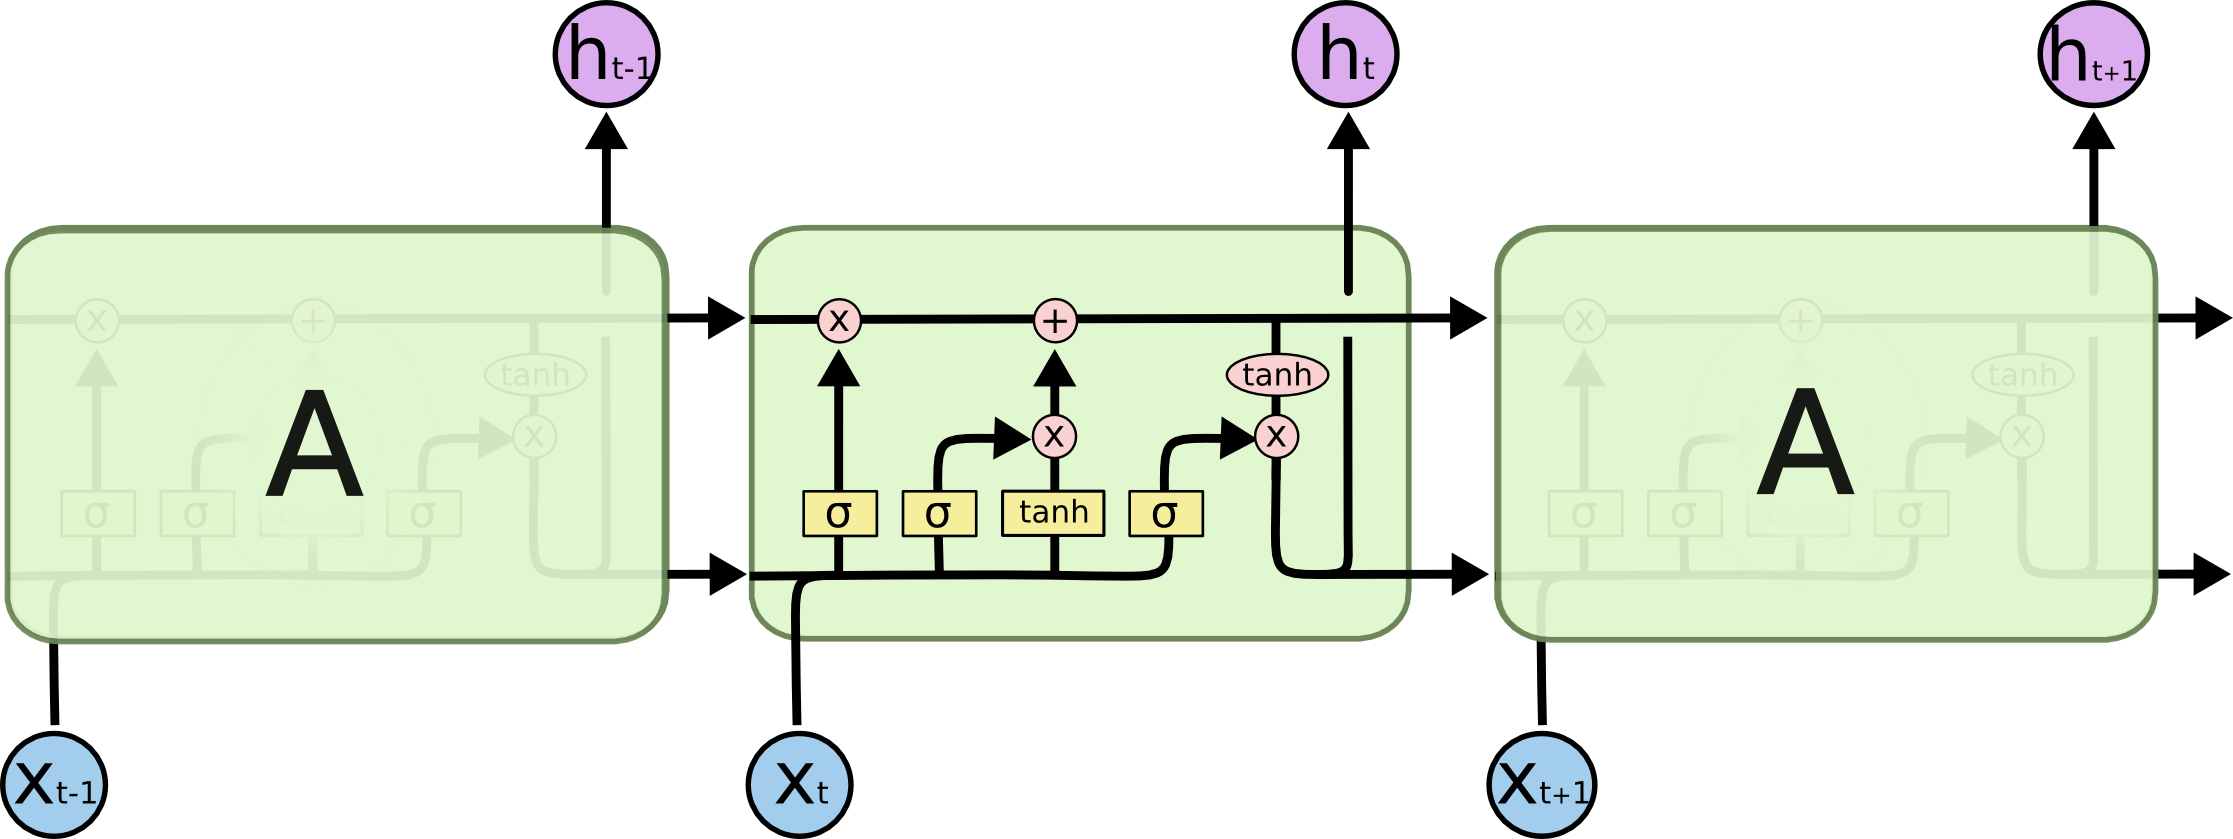
\includegraphics[width=0.8\textwidth]{images/LSTM3-chain.png}
\caption{LSTM Chain cell}
\label{fig:lstmcell}
\end{figure}

Using LSTMs have proved very successful as seen in Machine Learning tasks such as \cite{Sutskever2014}. Additional usage of bidirectional features captures past and present memory of features inherent in training data as seen in \cite{Graves2005} for phoneme classification. Using both concepts lead to Bidirectional LSTM usage with a CRF layer as seen in \cite{Lample2016} which showed state of the art results in a completely data driven approach to NER. 

\section{Discussion}
A well adapted system to perform the \dimsum task will require the ability to assign useful semantic tags to lexical items and heterogeneous MWEs. This entails the ability to recognise weak and strong MWE constructions with ``gappy'' structures. Statistics drawn from \cite{Schneider2014} show that around 75\% of constructions are strong, i.e. {\bf Fixed Expressions} or {\bf Institutionalised Phrases}, but the additional 25\% are weak being {\bf Semi-Fixed Expressions} or {\bf Syntactically-Flexible Expressions}. Choosing to ignore these ``gappy'' constructions shows ``loss in performance''\cite{Schneider2014} which is to be expected. As seen previously, \cite{Ramisch2012} confirms that coverage of a specific lexical category can be modelled to have high coverage but low overall performance\footnote{``Cover most of the nominals... having lower precision'' \cite{Ramisch2012}}. 

It is a pervasive belief that semantic senses are common across languages whereas lexical features are not. For a robust and generalised system, a scope which encompasses supersenses on lexical items should be used. Ideally, being portable and scalable are equally important which implies elegant algorithms and availability of labelled data or more intricate models with unlabelled data. At this point, state-of-the art systems rely on structural data. 
Therefore, the initial baseline for \dimsum should include these features that capture structure and generalise meaning well. This should include multi-category MWE recognition and supersense tagging. 

Since there are many research topics that lead to positive results using CRFs, initial baseline construction will follow suit. In addition, a network architecture approach using LSTMs will be created in addition. More details on design can be read about in Chapter \ref{chapter4}.

